\chapter{Asking Supercar Owners How They Got RICH! (Florida)}

These notes follow a School of Hard Knocks field lecture, curated by LazyingArt LLC, as a sequence of operating rules extracted from public interviews with wealthy business owners in Tampa. There is no blackboard here, but there is still a mathematical spine. We are given a city-level quantitative claim, a simple liquidity equation, a filter for deciding whose advice counts, a model of why crowded markets may still be open, a sales rule based on assuming the close, and finally a bargaining picture in which leverage rises when one can walk away. The material is best read not as abstract motivation but as a chain of local models, each introduced by the same ritual: identify the asset, identify the business, identify the scale, and then ask what rule survived contact with reality.

\section{Tampa as a Field Site}

The lecture opens with a teaser reel: expensive cars, scattered income claims, and several hard-edged lines about money, risk, and work. That opening does not yet argue anything; it promises that visible wealth will be translated into explicit operating rules. The real setup begins when the host names Tampa as a city dense with visible capital and treats the city itself as a sample space.

The governing numerical claim is presented immediately:
\begin{equation}
N_{\text{millionaires}}(\text{Tampa}) > 50{,}000.
\end{equation}
The chapter should keep this as the host's framing claim rather than as an independently verified demographic theorem. Its function is motivational and methodological: if we walk through an environment that is supposedly rich in successful operators, we may expect repeated local rules rather than a single heroic biography.

What follows is therefore not one long argument by one speaker. It is a sequence of entrepreneurial micro-lectures. Each begins with an object of status, then a business identity, then a time scale, then a revenue scale, and only then turns to mechanism. The rhythm matters. Credential comes before doctrine.

\section{Interview One: Advice, Liquidity, and Competitive Markets}

The first full interview begins with a Rolls-Royce owner who identifies himself as a healthcare entrepreneur and says he owns the largest medical sleep testing company in the United States. He places himself on a long time horizon,
\[
t_{\text{biz,health}} \approx 28\ \text{years},
\]
and gives a peak earning description of ``multiple eight figures.'' Only after this credentialing does the host turn to the central question: what advice survives that scale and that duration?

\begin{definition}
Fix a domain
\[
d \in \{\text{money},\text{business},\text{relationship},\text{friendship}\}.
\]
A transcript-faithful formalization of the speaker's rule is the \emph{advice filter}: retain advisor \(i\) only when \(i\) has demonstrated superior outcomes in that same domain. In symbols,
\begin{equation}
O_d(i) > O_d(j)
\end{equation}
means that advisor \(i\) dominates advisor \(j\) in the relevant domain \(d\), and therefore \(i\) is the more credible source of advice.
\end{definition}

The speaker states the rule in plain language: do not take money advice from people who make less money than you, do not take business advice from people with smaller businesses, do not take relationship advice from people with failed marriages, and do not take friendship advice from people with no friends. The transcript becomes garbled in the friendship line, but the intended structure is clear. We are not being given a democratic theory of counsel. We are being given a performance filter.

The next move is important. The speaker does not leave the rule floating in abstraction. He immediately grounds it in a brokenness anecdote: nine years earlier he had \(\text{\$}78\) in the bank. He sharpens the point by specifying that this was the \emph{available} balance, not a ceremonial number. That gives us a very simple balance equation:
\begin{align}
B_{\text{avail}} &= \text{\$}78,\\
B_{\text{post}} &= B_{\text{avail}} - C_{\text{out}},
\end{align}
where \(C_{\text{out}}\) denotes outstanding checks or near-term obligations. The operational danger is then immediate:
\begin{equation}
C_{\text{out}} > \text{\$}78 \quad \Rightarrow \quad B_{\text{post}} < 0.
\end{equation}

This is elementary arithmetic, but it matters because the lecture is careful about the difference between being poor in a vague emotional sense and being one payment away from operational failure.

\paragraph{Worked example.}
As a purely illustrative update, suppose a pending obligation arrives in the amount of \(\text{\$}100\). Then
\begin{equation}
B_{\text{post}}=\text{\$}78-\text{\$}100=-\text{\$}22.
\end{equation}
The speaker's point is not the number \(\text{\$}100\) in particular; it is that low liquidity makes even ordinary obligations dangerous. The business problem is not merely low wealth. It is low buffer.

The host then asks what sets this operator apart in a highly competitive healthcare industry, and the first speaker gives the lecture's most explicit market argument. His claim is that competition should not frighten us by itself. A competitive industry is evidence that there is a lot of money in the arena. The further claim is quantitative:
\begin{equation}
p(R>\text{\$}10\,\mathrm{M}) < 0.01.
\end{equation}
He also says something like ``it's like \(0.07\),'' but the exact normalization is unclear, so the safe lesson is only that the upper tail is very small.

A clean way to write the underlying idea is
\begin{equation}
N_{\text{elite}} = p_{\text{elite}}N, \qquad p_{\text{elite}} \ll 1,
\end{equation}
where \(N\) is the total number of participants in the market and \(N_{\text{elite}}\) is the very small subset willing to execute at an extreme level. The lecture's rhetoric is rougher than this. The structure, however, is precise: large markets can be crowded at the entrance and thin at the frontier.

\begin{proposition}
A crowded market is not necessarily closed to a disciplined entrant.
\end{proposition}

\begin{proof}
Suppose many firms participate, so \(N\) is large. If only a small upper-tail fraction \(p_{\text{elite}}\) actually sustains the effort, discipline, and execution required to reach serious scale, then the effective frontier contains only \(N_{\text{elite}}=p_{\text{elite}}N\) competitors, with \(p_{\text{elite}}\ll 1\). Thus crowding at the surface and openness at the frontier can coexist. This is the mathematical skeleton of the interviewee's claim that one can still dominate a ``competitive'' industry by working at a level most entrants will not sustain.
\end{proof}

\subsection{Question \& Answer}

\paragraph{Question.} Why does the speaker become more excited, not less, when he hears that an industry is competitive?

\paragraph{Answer.} Because in his model competition is evidence of market size, not proof of saturation. The hidden variable is not how many people enter, but how few remain at the top of the effort distribution. The lecture's resolution is therefore not ``avoid crowded markets.'' It is ``distinguish the crowd from the true frontier.''

\begin{figure}
\centering
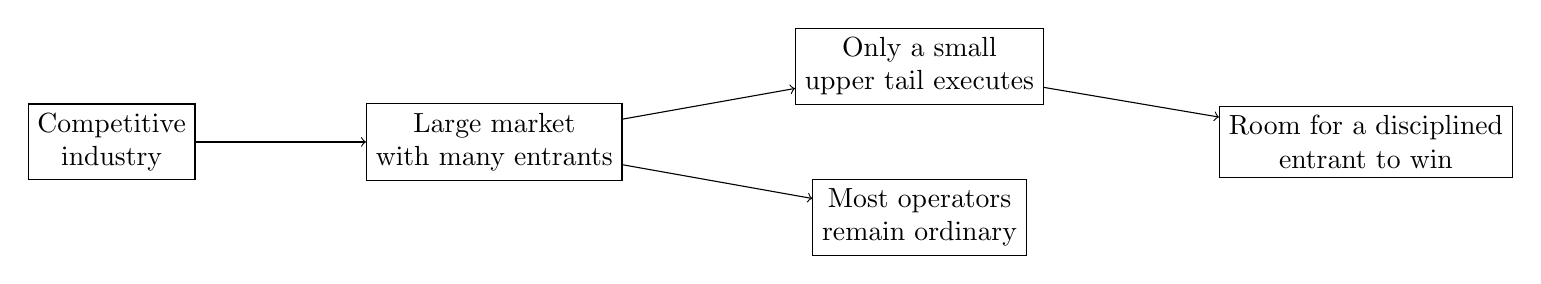
\begin{tikzpicture}[x=2.7cm,y=1.2cm]
\node[draw,rectangle,align=center] (a) at (0,0) {Competitive\\industry};
\node[draw,rectangle,align=center] (b) at (1.8,0) {Large market\\with many entrants};
\node[draw,rectangle,align=center] (c) at (3.8,0.8) {Only a small\\upper tail executes};
\node[draw,rectangle,align=center] (d) at (3.8,-0.8) {Most operators\\remain ordinary};
\node[draw,rectangle,align=center] (e) at (5.9,0) {Room for a disciplined\\entrant to win};
\draw[->] (a) -- (b);
\draw[->] (b) -- (c);
\draw[->] (b) -- (d);
\draw[->] (c) -- (e);
\end{tikzpicture}
\caption{A transcript-derived map of the first interview's central market argument.}
\end{figure}

The host then compresses the first case into a public lesson: near-zero liquidity can be overcome, but not by fantasy. The recap stresses delegation, selling, work, and a long climb from \(\text{\$}78\) to large-scale enterprise. That recap matters. It tells us how the lecture itself wants the anecdote to be read.

\section{Interview Two: Sales Presupposition and Entrepreneurial Selection}

The second major interview again starts with credentialing. The car is another Rolls-Royce. The speaker runs a hedge fund for digital assets, says he has been in business for roughly a decade, and gives a peak-year income of
\begin{equation}
R_{\text{peak,hedge}}=\text{\$}4.5\,\mathrm{M}.
\end{equation}
Only then do we move to mechanism.

The host asks for the best sales and negotiation advice for people struggling to close deals. The answer is short and memorable: assume the close. The speaker immediately glosses the phrase: speak to the other person as if they are already your client. Then he adds a second variable: make the person laugh. The lecture's informal probability model is therefore
\begin{equation}
P(\text{close}\mid \text{assume close},\ \text{rapport})
>
P(\text{close}\mid \text{neutral framing},\ \text{low rapport}).
\end{equation}
This should not be overstated as measured evidence. It is the speaker's working sales heuristic. But it is a real model. Framing matters, and liking matters.

We may say the rule has two stages. First, remove the posture of pleading by presupposing a future commercial relationship. Second, reduce resistance by generating positive affect. In the speaker's own wording, people do not like to say no to someone they like.

The lecture then shifts abruptly from conversion to fragility. Asked about the lowest point in his career, the speaker describes litigation by large corporations over one of his companies. He says he won and that business insurance covered much of the burden. This gives us a structural reminder: good sales technique does not abolish downside. The operating business remains exposed to legal and contractual risk, and one of the lecture's cleanest prescriptive lines follows:
\begin{itemize}
\item sell hard,
\item but insure the business,
\item because adverse events do not ask whether one is charismatic.
\end{itemize}

The host then asks whether everyone can be an entrepreneur, and the answer is absolute: no. The reasoning is also precise. Entrepreneurship is described as repeated obstacle-clearing under high stress. The job is not one large act of inspiration; it is the constant fixing of problems under uncertainty.

\subsection{Question \& Answer}

\paragraph{Question.} If sales skill and work ethic matter so much, why does the speaker still insist that entrepreneurship is not for everyone?

\paragraph{Answer.} Because in this lecture entrepreneurship is not defined by desire alone. It is defined by repeated exposure to uncertainty, legal risk, volatile income, and the duty to solve problems without collapse. The second speaker therefore adds a selection principle to the first speaker's optimism. Large rewards exist, but stress tolerance is part of the entry requirement.

The interview ends with the host asking how somebody gets a Rolls-Royce in the present world. The answer is a blunt compression of the entire segment: work, reinvest, and stop looking for magic. The host's recap again matters because it names the extracted lesson directly. The lecture wants us to see this case not merely as a success story but as a filter: this path is available, but it is not soft.

\section{Interview Three: Confidence, Marriage, Faith, and Money Discipline}

The third interview widens the causal frame. The speaker identifies herself simply as an entrepreneur, says she has been a business owner since \(2019\), reports a best year of
\begin{equation}
R_{\text{peak,woman}}=\text{\$}2.5\,\mathrm{M},
\end{equation}
and says she has also been broke several times before hitting her stride. The lecture does not linger here on car ownership or negotiation tactics. Instead it asks what she would say to her twenty-year-old self.

The answer is to believe in oneself. But again the lecture does not leave the answer in the air. The next question asks how such belief was actually found, and the response is concrete: her husband. The support structure is externalized. Self-belief is not treated as pure inner alchemy; it is stabilized by a close relational partner who pushes action, risk, and trial.

That naturally leads to a second question: how important is it to marry the right person? Her answer is that this is one of the most important decisions because the wrong partner pulls one in the opposite direction of one's intended life.

The next layer is faith. She describes faith as her backbone, the thing she relies on day by day. Then, when asked for the best financial advice she has received, she gives a compact rule against overextension and adds that money should work for you rather than against you. A clean formalization, stated cautiously, is
\begin{equation}
\text{Overextension}\uparrow
\qquad \text{as} \qquad
\frac{\text{fixed obligations}}{\text{cash flow}} \uparrow.
\end{equation}
This equation is not spoken in the lecture, but it faithfully captures the operational meaning of her advice. When fixed commitments grow faster than reliable cash generation, money ceases to serve and begins to dictate. The deeper point is not moralistic thrift. It is structural control.

We should notice the pace here. After the first two interviews, which emphasize selection, aggression, competition, and sales, the lecture inserts a softer but equally rigorous causal layer: who stands behind the entrepreneur, what emotional architecture sustains action, and how does one keep finance from turning into a machine that owns the owner?

\section{Interview Four: Hunger, Silence, Leverage, and Power}

The last major interview is the widest in scope. The speaker identifies himself as a lobbyist and publicist with a consulting practice. He says he has been at it for nearly fifteen years,
\[
t_{\text{biz,lobby}} \approx 15\ \text{years},
\]
reports a peak year of
\[
R_{\text{peak,lobby}}=\text{\$}1.4\,\mathrm{M},
\]
and immediately adds the caveat that the following year he nearly lost everything while trying to scale an agency. The lecture thereby repeats a central motif: peak visible income is not the whole story. Fragility shadows scale.

Asked whether he could rebuild if he went broke tomorrow, he says yes, and the justification is hunger. He has already lived close to the floor. He describes sleeping rough, choosing between transit and food, and doing hard labor before launching his company. This is a resilience model. If one can lower the consumption floor and retain willingness to work, then downside loses some of its power to terrify.

He then dates his own milestones:
\begin{align}
a_{\text{current,lobby}} &= 38,\\
a_{\text{millionaire,lobby}} &= 35.
\end{align}
This matters because the lecture is not presenting overnight ascent. Again we have a multi-year build with low-status work before recognizable success.

The host asks for the best advice from a mentor, and now two maxims appear. First: never let them see you sweat. Second: do not believe your own propaganda. The first is about public composure under pressure. The second is about internal discipline under success. The speaker illustrates both with a long anecdote about making money quietly while appearing externally unimpressive, precisely to avoid hostility and premature attention. This is an argument for moving in silence.

Only after this psychological and reputational framing does the lecture return to explicit sales technique. Asked about the secret to sales in a competitive industry, he answers: be able to walk away. Here the mathematical core is leverage:
\begin{align}
O_{\text{outside}} \uparrow &\Rightarrow L_{\text{bargain}} \uparrow,\\
\text{Neediness} \uparrow &\Rightarrow L_{\text{bargain}} \downarrow.
\end{align}
The speaker then adds a sharper heuristic: the first person to speak loses. We should not universalize that as a law of bargaining theory, but we can hear its function. He wants to replace the posture of chasing a deal with the posture of presenting value: consistency, case studies, cadence. If the client wants cheap, let the client go elsewhere.

\subsection{Question \& Answer}

\paragraph{Question.} What actually creates leverage in a competitive sales or political environment?

\paragraph{Answer.} In the lecture's final model, leverage is not noise, aggression, or theatrical self-belief. It is a combination of demonstrated value and a credible outside option. One wins not by needing the deal more loudly, but by needing it less and proving the worth of one's terms more clearly.

The interview then widens from individual bargaining to public structure. Asked whether politicians are corrupt, the speaker shifts the frame and says power corrupts. Asked about the biggest lie told by government, he denies the simple fantasy that one can merely ``drain the swamp'' and instead argues that bureaucrats and lobbyists carry durable institutional knowledge. These are strong claims and should remain clearly attributed to the speaker. They are not formal political science results. But they do continue the lecture's underlying theme: what matters most is rarely the surface spectacle. One must identify the durable operating machinery beneath the public performance.

The final questions turn to faith, and the speaker answers in explicitly Christian language. In the lecture's sequencing, that matters. We move from hunger, to self-command, to leverage, to institutional power, and only then to theology. The effect is to present faith not as a substitute for technique but as a final layer underneath it.

\section{Summary}

The chapter begins with spectacle and ends with structure. In between, four interviewees generate a small bank of transcript-backed operational rules:
\begin{itemize}
\item filter advice by domain-specific results;
\item remember that low liquidity is a hard equation, not a mood;
\item do not confuse market crowding with frontier closure;
\item assume the close, but protect the business;
\item do not universalize entrepreneurship, because the path selects for stress tolerance;
\item cultivate support structures that strengthen confidence rather than weaken direction;
\item do not overextend;
\item preserve leverage by being able to walk away.
\end{itemize}

What makes the lecture usable is its rhythm. Wealth is shown first, then interrogated, then reduced to mechanism. The cars are the bait. The notes must keep the machinery.